\chapter{Machine Learning Methods Applied to Synthetic Ion Acceleration Data} \label{ch:5}

In recent years, the application of \gls{ML} methods to \gls{HEDS} has exploded due to two main reasons. First, ultra-intense laser systems are now capable of firing many shots per second and collecting data at a similar rate. This allows scientists to collect a lot of data, which cannot reasonably be handled in real-time by a human. Second, machine learning frameworks like PyTorch \cite{PyTorch_2019} are easily accessible and powerful so that scientists who are not machine learning researchers are capable of using them.

One approach to applying machine learning with a limited amount of data is \gls{BO}. \GLS{BO}, based on prior collected data points, attempts to find another suitable data point that is different than the prior data and expected to yield a more optimized output (according to some chosen criteria). Using \gls{BO}, Jalas et al. \cite{Jalas_2021_PRL} optimizes the quality of a laser-accelerated electron beam and Dolier et al. \cite{Dolier_2022_NJoP} optimizes the maximum proton energy using PIC simulations. Another notable effort is Loughran et al. \cite{Loughran_2023_HPLSE} who used this approach to demonstrate higher maximum cutoff proton energies from an experiment using a 1 Hz laser. While this approach is commendable, it does not scale well to laser repetition rates of 100 or more Hz. 

Quite a few works have explored using neural networks to analyze and extract information from large datasets generated from \gls{PIC} simulations. Djordevic et al. \cite{Djordjevic_2021_PPCF} used these simulations to find an empirical estimate for the effective acceleration time by using a \gls{NN} model (which informs our choice of 1.3 in \autoref{eq:fuchs_multiplier}). Schmitz et al. \cite{Schmitz_2023_LaPB} also trained \gls{NN}s on \gls{PIC} simulation data to better understand optimal laser and target parameter combinations for their system at TU Darmstadt. One thing these studies have in common is that they only use data from \gls{PIC} simulations which don't necessarily reflect real experiments (especially so because they are 1D and 2D simulations with reduced dimensionality). 

The \gls{WP-ELL} has a (1 kHz, $\tau_\text{FWHM} = 40$ fs, $\lambda = \SI{0.8}{\micro \meter}$, $w_0 = \SI{1.5}{\micro \meter}$) mJ class laser that can currently collect ion spectrometer data at a maximum rate of 100 Hz \cite{George_2019_HPLSE}. The laser irradiates a liquid target, formed from the intersection of two flowing liquid streams, that can be sustained for around 45 minutes before needing to be refilled. This acquisition rate and time could theoretically result in 270,000 unique data points during one collection. Laser systems like this are still new and the stability of the liquid target often interferes with the goal of collecting quality data. As a result, we first focused our energy into doing a \gls{ML} analysis on data produced from a well-known model by Fuchs \cite{Fuchs_2005_Nat} based on parameters at \gls{WP-ELL}. The goal of this analysis is not to make recommendations on what input parameters should be used in experiment, but to provide a general framework that can be extended to real data and also to help others incorporate \gls{ML} in their work by sharing our code (see Zenodo \cite{Desai_2024_Zenodo, Desai_2025_Zenodo} for the python code and datasets). By providing these files we hope to encourage others to compare other ML models against our results as a benchmark. This chapter details the work I did developing this synthetic dataset, comparing different \gls{ML} algorithms, and evaluating their potential effectiveness in a real experiment. 

\section{Modified Fuchs et. al. Model} \label{sec:fuchs_model}

In this section, I will describe the model from which we generated the synthetic datasets \cite{Desai_2024_CPP, Desai_2025_APL}. First, the expansion of a plasma into a vacuum \cite{Mora_2003_PRL} is used to determine the maximum proton energy and the number of accelerated protons per unit energy $\frac{dN}{dE}$. Following Fuchs \cite{Fuchs_2005_Nat}, we define the acceleration time in proportion to the pulse duration of the laser and adopt a scaling (e.g. \autoref{eq:wilks}) to relate hot electron temperature to the ponderomotive potential. This, in combination with other empirical estimates, allows calculating a proton energy spectrum from up to 7 parameters: main pulse intensity, contrast, wavelength, pulse duration, target thickness, target focal position, and laser spot size.

\subsection{Plasma Expansion into a Vacuum}

This model was developed by Mora \cite{Mora_2003_PRL} in 2003 who built off of earlier efforts \cite{Crow_1975_JPP,Kishimoto_1983_PoF} in examining an isothermal expansion model. The model begins with the assumption that ions are contained in the semi-infinite interval $n_i = n_{i0}$ for $x < 0$ and no ions are initially in the vacuum region for $x > 0$. The electrons are distributed according to the boltzmann relation given by \autoref{eq:boltzmann} where $n_{e0} = n_e(x = -\infty)$ is the electron density in the unperturbed plasma. Through this relation, $\phi(-\infty) = 0$. The initial electron density is related to the ion density $n_{e0} = Z n_{i0}$ where $Z$ is the ion charge number for a fully ionized plasma. The potential also satisfies the Poisson equation \autoref{eq:poisson} where $\rho/m = - e (n_e - Z n_i)$. The solution of \autoref{eq:poisson} at $t=0$ is found by integration \cite{Crow_1975_JPP} (where $E \equiv -\frac{d\phi}{dx}$) as 

\begin{equation}
	\frac{1}{2} \epsilon_0 E^2 = n_{e0} k_B T_e
	\begin{cases}
		\exp(\frac{e \phi}{k_B T_e} - 1 - \frac{e \phi}{k_B T_e}) & \mbox{if x < 0} \\
		\exp(\frac{e \phi}{k_B T_e}) & \mbox{if x > 0} \label{eq:crow_field}
	\end{cases}
\end{equation} 
From enforcing continuity of \autoref{eq:crow_field} at $x=0$ (the location of the ion front initially) we determine $\phi = -k_B T_e / e$ to arrive at  

\begin{equation}
	E_{front,0} = \sqrt{\frac{2}{\exp(1)}} E_0
\end{equation}
where $E_0 \equiv \sqrt{n_{e0} k_B T_e / \epsilon_0}$. To get an estimate of the electric field at the ion front when $t > 0$ we need to consider what the characteristic time scale for ion motion is: the plasma ion frequency $\omega_{p,i}$

\begin{equation}
	\omega_{p,i} \equiv \sqrt{\frac{Z n_{e0} e^2}{m_i \epsilon_0}}	\label{eq:omegapi}
\end{equation} 
which is analogous to \autoref{eq:omegape}. In relation to the time-scale of plasma ion oscillations, a long time would refer to $\omega_{p,i} t \gg 1$. The ion fluid sound speed $c_s$ is given by 

\begin{equation}
	c_s = \sqrt{\frac{Z k_B T_e}{m_i}} \label{eq:soundspeed}
\end{equation}
which is very similar to \autoref{eq:vthermal} Using the definition of the debye length (\autoref{eq:debye}) and sound speed $c_s$ we can re-express \cref{eq:omegapi} as 

\begin{equation}
	\omega_{p,i} t = \sqrt{\frac{Z k_B T_e}{m_i}} \sqrt{\frac{n_{e0} e^2}{\epsilon_0 k_B T_e}} t = (c_s t) (\lambda_{D0})
\end{equation}
where $\lambda_{D0}$ is the initial Debye length and $c_s$ is the ion sound speed. As we know from \autoref{ch:2}, when $\lambda_D$ is smaller than the characteristic length scale of a system, the quasi-neutrality condition for a plasma is satisfied. In this case, the length scale would be $c_s t$ and we can show that asserting the condition $\omega_{p,i} t > 1$ is equivalent to $\lambda_D < c_s t$. We can continue by incorporating equations of continuity and the Lorentz force (\autoref{eq:lorentz}) which can be expressed as 

\begin{subequations}
	\begin{align}
		\frac{\partial n_i}{\partial t} + v_i \frac{\partial n_i}{\partial x} &= - n_i \frac{\partial v_i}{\partial x} \label{eq:continuity} \\
		\frac{\partial v_i}{\partial t} + v_i \frac{\partial v_i}{\partial x} &= -\frac{Z e}{m_i} \frac{\partial V}{\partial x} \label{eq:lorentz_mora}
	\end{align}
\end{subequations}
This set of fluid equations can be solved numerically with the initial conditions for $n_i$, $E$, and $v_i = 0$, but it is more instructive to consider a \emph{self-similar solution} that describes the ions moving with speed 
\begin{equation}
	v_i = c_s + x/t \label{eq:selfsimilarvelocity}
\end{equation}
for $x + c_s t > 0$. It is self-similar in the sense that the specific length and time scales are not important, only their ratio $x/t$. In this self-similar region, quasi-neutrality is maintained and the expanding electron density can be expressed as

\begin{equation}
	n_e = Z n_i = n_{e 0} \exp(-\frac{x}{c_s t} - 1) \label{eq:selfsimilardensity}
\end{equation} 
By combining \cref{eq:continuity,eq:lorentz_mora,eq:selfsimilarvelocity,eq:selfsimilardensity}, we can arrive at a solution for the self-similar electric field in this quasi-neutral region

\begin{equation}
	E_{SS} = \frac{m_i c_s}{Z e t} = \frac{k_B T_e}{e c_s t} = \frac{E_0}{\omega_{p,i} t} \label{eq:selfsimilarefield}
\end{equation}
Physically, we can interpret this as a sheet of positive charge $\sigma = \epsilon_0 E_{SS}$ at $x = - c_s t$ and a sheet of negative charge $-\sigma$ at the plasma edge. The location of this plasma edge (i.e. the location of the ion front) can be roughly obtained by equating the local Debye length $\lambda_D = \lambda_{D0} \sqrt{n_{e0}/n_e}$ to the scale length $c_s t$.

\begin{equation}
	x_{i, front} = c_s t [2 \ln(\omega_{p,i} t) - 1] \label{eq:mora_xfront}
\end{equation} 
and the ion velocity at the front can also be obtained 

\begin{equation}
	v_{i, front} = 2 c_s \ln(\omega_{p,i} t)
\end{equation}
The ion velocity can be plug back into \autoref{eq:lorentz_mora} to find out that $E_\text{front,SS} = 2 E_{SS}$. Mora found an approximate solution to $E_{front}$ that matches $E_\text{front,0}$ and $E_\text{front,SS}$ in their respective cases ($t = 0$ and $\omega_{p,i} t \gg 1$) as 

\begin{equation}
	E_{front} \simeq \frac{2 E_0}{\sqrt{2 \exp(1) + (\omega_{p,i} t)^2}}
\end{equation}
This formula not only reaches the correct values in the limiting cases, but also effectively interpolates in the intermediary regions (i.e. $\omega_{p,i} t \sim 1$) when compared to a numerical code that solves \cref{eq:continuity,eq:lorentz_mora} without assuming a self-similar solution. In \autoref{fig:fig1_mora}, we see the net charge density at some time $\omega_{pi} t = 50$ after the start of a 1D plasma expansion simulation. We can identify the $-2\sigma$ with the fastest expanding electrons and the $+\sigma$ region next to it as the positive ions getting pulled along. In \autoref{fig:fig2_mora}, we can see the electric field between these two charged regions peaks $\simeq 2 E_{ss}$. Then, using this formula with $\autoref{eq:lorentz_mora}$, we can determine the ion front velocity as 

\begin{figure}
	\centering 
	\subfloat{
		\label{fig:fig1_mora}
		\includegraphics[width=0.5\linewidth]{planning/images/fig1_mora.PNG}
	}
	\subfloat{
		\label{fig:fig2_mora}
		\includegraphics[width=0.5\linewidth]{planning/images/fig2_mora.PNG}
	}
	\caption{The net charge density (left) as a function of position $x / c_s t$ and normalized electric field $E/E_0$ (right) for $\omega_{pi} t = 50$ taken from Fig 1 and 2 in Mora's Paper \cite{Mora_2003_PRL}. On the right, the self-similar electric field from \autoref{eq:selfsimilarefield} is plotted with a dashed line.}
\end{figure}

\begin{equation}
	v_{i,front} = 2 c_s \ln(\tau + \sqrt{\tau^2 + 1})	
\end{equation}
where we've defined a normalized acceleration time $\tau \equiv \omega_{p,i} t / \sqrt{2 \exp(1)}$. Additionally, in the limit $\omega_{p,i} t \gg 1$, \autoref{eq:mora_xfront} becomes

\begin{equation}
	x_{i, front} \simeq c_s t [2 \ln(\omega_{p,i} t) + \ln(2) - 3] \label{eq:mora_xfront_simple}
\end{equation}
The per-ion kinetic energy can now be calculated as

\begin{align}
	\mathcal{E} \equiv \frac{1}{2} m_i v_{i,front}^2 &= 2 m_i c_s^2 \ln(\tau + \sqrt{\tau^2 + 1})^2  \nonumber\\
	&= 2 Z k_B T_{e} \ln(\tau + \sqrt{\tau^2 + 1})^2 \label{eq:mora_maxE}
\end{align}
Using \autoref{eq:selfsimilardensity}, we can determine the number of accelerated ions between $x = -c_s t$ and $x = x$ as

\begin{equation}
	N_i \equiv \int_{-c_s t}^{x} n_i(x') dx' = n_{i0} c_s t [1 - \exp(-\frac{x}{c_s t} - 1)]
\end{equation}
and using \autoref{eq:selfsimilarvelocity}, we can show that this is equivalent to 

\begin{equation}
	N_i(x) = n_{i0} c_s t [1 - \exp(-\sqrt{\frac{2 \mathcal{E}}{\mathcal{E}_0}})] \label{eq:numprotons}
\end{equation}
where $\mathcal{E}_0 \equiv Z k_B T_e$. Now that the number of ions is expressed in terms of the energy $\mathcal{E}$, we can determine the number of accelerated ions per unit energy (per unit surface) as 

\begin{equation}
	\frac{d N}{d \mathcal{E}} = \frac{n_{i0} c_s t}{\sqrt{2 \mathcal{E} \mathcal{E}_0}} \exp(-\sqrt{\frac{2 \mathcal{E}}{\mathcal{E}_0}}) \label{eq:dNdE}
\end{equation}
	
\subsection{Modified Fuchs Model} \label{sec:fuchsv1}

When $\tau \rightarrow \infty$, \cref{eq:mora_maxE} diverges to $\infty$. This is an inherent limitation of the isothermal fluid model, and different models are able to avoid this issue \cite{Mora_2005_PRE,Passoni_2010_NJoP,Schreiber_2006_PRL}. However, a simple fix to this model involves assuming that this acceleration time is finite and proportional to the pulse duration. Physically, it makes sense that the protons are only getting accelerated on the timescale of  laser-target interactions. This is the approach taken by Fuchs \cite{Fuchs_2005_Nat} and he expresses \autoref{eq:mora_maxE} as 

\begin{equation}
	E_\text{max} = 2 k_B T_h [\ln(t_p + \sqrt{t_p^2 + 1})]^2 \label{eq:fuchs_maxE}
\end{equation}
where $t_p \equiv \omega_{p,i} t_\text{acc} / \sqrt{2 \exp(1)}$ just like the Mora model. We've also set $Z=1$ to signify that we are looking for hydrogen ions (i.e. protons) The crucial difference is that we express the acceleration time as 

\begin{equation}
	t_\text{acc} \approx 1.3 \tau_\text{FWHM} \label{eq:fuchs_multiplier}
\end{equation}
One can assume that the absorption fraction of hot electrons $\eta$ (with respect to the total laser energy $E_L$) is given by $\eta_e = 1.2 \times 10^{-15} I^{0.74} \text{ W cm}^{-2}$ with a maximum of 0.5, determined from empirical scalings (e.g. see fig. 3 from Key \cite{Key_1998_PoP}). Additionally, the average energy of the hot electrons is set by the Wilks scaling (\autoref{eq:wilks}). Putting this together, 

\begin{equation}
	N_e = \eta_e \frac{E_L}{T_h}
\end{equation}
would be the total number of hot electrons accelerated into the target. These electrons spread out in a roughly cylindrical volume of area $S_\text{sheath}$ and length $c \tau_\text{fwhm}$ where the circular sheath cross section can be estimated by $S_\text{sheath} = \pi (r_0 + d \tan(\theta))^2$. Here, $r_0 = w(x) \frac{\sqrt{2 \ln(2)}}{2}$ is the (spatial) half width at half maximum of the intensity distribution at position $x$. The effective radius of the sheath has an additional factor of $d \tan(\theta)$ where $d$ is the initial target thickness and $\theta$ is the half-angle divergence of the hot electrons within the target (taken as $\theta = 25^\circ$). As a result, the hot electron number density can be expressed as 
	
\begin{equation}
	n_{e0} = \frac{N_e}{c \tau_\text{fwhm} S_\text{sheath}}
\end{equation}
With an estimate of the hot electron density, the proton spectrum can now be computed from \cref{eq:dNdE} as 

\begin{equation}
	\frac{dN}{dE} = N_0 \frac{\exp(-\sqrt{2 E/k_B T_h})}{\sqrt{2 E k_B T_h}} \label{eq:dNdE_Fuchs}
\end{equation}
where $N_0 \equiv n_{e0} c_s t_\text{acc} S_\text{sheath}$ is defined for convenience. Using a dimensionless scale for energy $\varepsilon \equiv \sqrt{2 E / k_B T_h}$, we can calculate the number of protons and total energy in protons through integrating \autoref{eq:dNdE_Fuchs}

\begin{align}
	N &= N_0 (\exp(-\varepsilon_\text{min}) - \exp(-\varepsilon_\text{max})) \label{eq:fuchs_N} \\
	E_\text{tot} &= N_0 \frac{k_B T_h}{2}[\exp(-\varepsilon_\text{min})(2 + \varepsilon_\text{min}(2 + \varepsilon_\text{min})) - \exp(-\varepsilon_\text{max})(2 + \varepsilon_\text{max}(2 + \varepsilon_\text{max}))] \label{eq:fuchs_totE}
\end{align}
where $\varepsilon_\text{min} = \sqrt{2 E_\text{min} / k_B T_h}$ defines a minimum energy cutoff ($\varepsilon_\text{max}$ is analogous and chosen by \autoref{eq:fuchs_maxE}). Furthermore, we can calculate the average proton energy by dividing \autoref{eq:fuchs_N} from \autoref{eq:fuchs_totE}

\begin{equation}
	E_\text{avg} \equiv \frac{E_\text{tot}}{N} \label{eq:fuchs_avgE}
\end{equation}
The combination of Equations \ref{eq:fuchs_maxE} and \ref{eq:dNdE_Fuchs} have been tested across many of the early \gls{TNSA} experiments of the early 2000s for a wide range of laser intensities and pulse durations with good accuracy (see fig. 4 from Fuchs \cite{Fuchs_2005_Nat}).

\subsection{Further Model Modifications} \label{sec:fuchsv2}
When restricted to a particular laser system, the wavelength, pulse duration, and spot size are fixed. Considering the model in \autoref{sec:fuchsv1}, only three adjustable parameters would be of interest -- target thickness $d$, peak intensity $I_0$ and target focal position $x$. To introduce complexity into our model, we wanted to consider the effect that a pre-expanded target would have on the proton acceleration. The pre-expansion may enhance the hot electron generation, but expansion on the rear side of the target would reduce the effectiveness of the \gls{TNSA} process. We incorporate this effect by allowing the laser to have a finite contrast $\kappa$ which relates the intensity of the main laser pulse $I_0$ to the intensity of a secondary laser pre pulse as $I_\text{pre} = \kappa I_0$. This pre-pulse is treated as a spike in intensity that occurs $t_0$ before the arrival of the main pulse. The pre-expanded target would have a new effective thickness given by 

\begin{equation}
	d_\text{eff} = d + 2 c_s t_0 \label{eq:d_eff}
\end{equation}
where $c_s$ is the ion sound speed from \cref{eq:soundspeed} in which the target is expanding outwards from both sides. Here $T_e$ is the temperature due to the pre-pulse and can be calculated by assuming that $T_e \propto I$ and that an intensity of $10^{12} \text{ W cm}^{-2}$ produces electron temperatures of $T_\text{pre,0} = 50$ eV. Since $n_e$ decreases as $d$ gets larger and $\omega_{p,i} \propto \sqrt{n_e}$, \autoref{eq:fuchs_maxE} is inversely proportional to the target thickness. So, a larger prepulse with a longer time to expand $t_0$ will see a higher effective target thickness. Furthermore, when the target is off focus, the effective pre-pulse intensity on target is less which results in less expansion.

In addition, some of the main pulse energy can be depleted by traveling through the underdense region of this new pre-expanded target. These effects will be referred to as \emph{pump depletion} and are inspired by arguments from Decker \cite{Decker_1996_PoP}. Decker describes pump depletion as an \emph{etching} process where traveling through the plasma causes wavefront edge to recede at a speed given by the \emph{etching velocity} 

\begin{figure}
	\centering 
	\includegraphics[width=0.6\linewidth]{planning/images/density_profile.png}
	\caption{The electron density profile of the pre-expanded target is depicted for various times $t_0$. In this figure, $n(0) \equiv n_\text{max}$. Taken from Desai et al. \cite{Desai_2025_APL} where $z$ was used as the distance along the laser axis instead of $x$ as done in this work. }
	\label{fig:density_profile}
\end{figure}
\begin{equation}
	v_\text{etch} = (\omega_{p,e}/\omega)^2 c \label{eq:vetch}
\end{equation}
Note that this speed continuously changes throughout the exponential-scale electron density which falls off like $n \sim \exp(-x/c_s t_0)$ on both sides of the target (see \autoref{fig:density_profile} for a visual). Due to conservation of particle number, if the target expands, the maximum density $n_\text{max}$ will also lower and is given by $n_\text{max} = \frac{n_{e0} d}{d_\text{eff}}$. We can integrate $v_\text{etch}$ with respect to time, but it is more convenient in terms of the position since we know the range over which the under-dense plasma exists. The plasma edge $x_f$ is given by \autoref{eq:mora_xfront_simple} and we will integrate up to the location of the critical density $x_0 = c_s t_0 (\ln(n_\text{max}) - \ln(n_c))$. Utilizing the change of variables $dx = c dt$ (due to the pulse traveling at the speed of light $c$), the ``etching distance'' can be calculated as \cite{Desai_2025_APL} 

\begin{equation}
	L_\text{etch} \equiv \int_{x_0}^{x_f} v_\text{etch} \frac{1}{c} dx = \frac{e^2 n_\text{max} c_s t_0}{\epsilon_0 m_e \omega^2} \left( \exp{\left(-\frac{x_0}{c_s t_0}\right)} - \exp{\left(-\frac{x_f}{c_s t_0}\right)} \right)
\end{equation}
Finally, this etching reduces the effective pulse duration by 

\begin{figure}
	\centering 
	\includegraphics[width=0.6\linewidth]{planning/images/energy_dip_morrison.png}
	\caption{The dotted black line shows the maximum proton energy predicted by \autoref{eq:fuchs_maxE} with the pump depletion considerations in \autoref{sec:fuchsv2} assuming $t_0 = \SI{60}{\pico \second}$, $I_0 = 10^{19} \text{W cm}^{-2}$, $\kappa=10^{-7}$, $d=\SI{0.5}{\micro \meter}$. The red stars indicate the predicted positions of maximum proton energy $\sim \SI{12}{\micro \meter}$. This plot is overlayed on top of an experimental maximum proton energy distribution from Morrison et. al. \cite{Morrison_2018_NJoP}. This figure is taken from Desai et. al. \cite{Desai_2025_APL}.}
	\label{fig:energy_dip_morrison}
\end{figure}
\begin{equation}
	\tau_\text{fwhm,eff} = \tau_\text{fwhm} (1 - \frac{L_\text{etch}}{c \tau_\text{fwhm}}) \label{eq:tau_etch}
\end{equation}
This model, however, is not without its flaws. First, our calculations assume a critical density of a tenth of the amount of the actual critical density. Second, instead of defining $d_\text{eff} = d_0 + 2 x_0$ (which would be the true effective density that remains above critical density), we substitute it with \autoref{eq:d_eff}. Third, we modify the multiplier seen in \autoref{eq:fuchs_multiplier} from 1.3 to 25 which is a significant departure. Finally, the proportionality $T_e \propto I$ with $T_\text{pre,0} = 50$ eV is chosen arbitrarily. Despite these drawbacks, we obtain model predictions similar to what is seen in \autoref{fig:energy_dip_morrison} to account for the maximum proton energy dip at peak focus. The goal of creating this model modification is to add complexity to the underlying physics for the purposes of evaluating the effectiveness of machine learning models, not to invent new physics. 

\section{First Analysis} \label{sec:first_analysis}

In this section, the results from my publication in \emph{Contributions to Plasma Physics} \cite{Desai_2024_CPP} in November of 2024 will be discussed. This project started with the work of Joe Smith and Ricky Oropeza who first coded up the modified Fuchs et al. model in Python. Then, undergraduate student Tom Zhang did some preliminary work in exploring different \gls{ML} frameworks to see what models could fit the data the best with some contributions from an another undergraduate student Pedro Gaxiola at \gls{CSUCI}. I initially worked in a complementary fashion to Tom, but finished up the project after Tom graduated from OSU with some help from undergraduate student Jack Felice. Along the way we were supported by coauthors Alona Kryshchenko from \gls{CSUCI} in addition to Anil Patnaik and Michael Dexter from \gls{AFIT}. This work was modeled on the \gls{WP-ELL} laser system described in et al. \cite{George_2019_HPLSE} with laser parameters mentioned in the beginning of \autoref{ch:5}.

\subsection{Methods}
In this work, we explored a 25,000 point dataset based on the model described in \autoref{sec:fuchsv1} which had three output quantities: $E_\text{max}, E_\text{tot}, E_\text{avg}$ (Equations \ref{eq:fuchs_maxE}, \ref{eq:fuchs_totE} \ref{eq:fuchs_avgE}). We modified the acceleration time (in \autoref{eq:fuchs_multiplier}) from 1.3 to 4 to better match the points in our dataset which is still within the range that Djordevic et al. \cite{Djordjevic_2021_PPCF} recommended.  Three input quantities were varied: peak laser intensity $I_0$ (from  $10^{18} \text{W cm}^{-2}$ to $10^{19} \text{W cm}^{-2}$), target thickness $d$ (from $\SI{0.5}{\micro \meter}$ to $\SI{10}{\micro \meter}$), and distance from peak focus to the target $x$ (from $\SI{-30}{\micro \meter}$ to $\SI{30}{\micro \meter}$). The input quantities were randomly chosen (uniformly within their intervals) with the Fuchs et al. model evaluations yielding the three outputs. To make the problem non-trivial, noise was added to the outputs sampled from a log-normal distribution with a mean of the output value and standard deviation between 0 and 30\% of the output value. Varying the noise, which would be present in an experimental dataset, will show how well a model can handle noise. Since we define the standard deviation as proportional to the mean (rather than some constant), the raw amount of noise becomes larger as the predictions get larger.

As a pre-processing step, we first applied a logarithm to both the intensity and three outputs of the model. This was necessary due to our choice of sampling the intensity uniformly with respect to the exponent (i.e. 18-19) and the output energies are directly proportional to the intensity. Additionally, we applied z-score normalization to both the inputs and outputs which is standard in machine learning algorithms to keep all data points on the same order of magnitude. From the 25,000 total points, we used 20,000 for training and reserved a hold-out set of 5,000 for testing. We determined the scalings from the training set only to ensure there is no leakage of information into the testing set. Furthermore, we multiplied the unscaled outputs by a correction factor equal to the mean of the training outputs divided by the unscaled outputs to reduce and under-predicting bias introduced by the log-scaling of the outputs \cite{Miller_1984_AmStat}.

We used three different \gls{ML} models in our study: \gls{SVR}, \gls{GPR}, \gls{NN} that were programmed using RAPIDS \cite{2023_RAPIDS}, GPyTorch \cite{Gardner_2018_GPytorch}, and Skorch \cite{Tietz_2017_Skorch} respectively in Python. These packages all contain functions to facilitate running \gls{GPU} accelerated scripts and were ran using the Pitzer cluster on the \gls{OSC}. All three approaches benefitted from hyperparameter optimization through the \texttt{GridSearchCV} module of scikit-learn. These choices are summarized in \autoref{tab:hps1}. For both the \gls{GPR} and \gls{SVR}, an \gls{RBF} kernel was used.

\begin{table}
	\centering
	\begin{tabular}{|c|c|}
			\hline
			NN & BS = 256, leaky ReLU, $N_h = 3$, $N_l = 64$, Adam, $\text{LR}=0.001$ \\
			\hline
			SVR & $\epsilon = 0.01$, $C = 2.5$, tolerance = $0.001$ \\
			\hline
			GPR & Iterations = 30, $\text{LR}=0.001$ \\
			\hline
	\end{tabular}
	\caption{Optimal hyperparameters found through grid searches and cross-validation using only the training set for the results in \autoref{sec:first_analysis}.}
	\label{tab:hps1}
\end{table}

\subsection{Results}

Our first task was to evaluate how well the trained models can fit the underlying dataset as the number of data points is increased. We accomplished this by evaluating the models on a testing set which is which is proportional to the amount of training points in a 80-20 training-testing split. In \autoref{fig:mape_3levels}, the \gls{MAPE} is evaluated between the model outputs and the testing data outputs to assess the accuracy of each method for three different noise levels -- 0, 15, and 30 \%. Since, in this figure, the testing data contains noise, it is impossible to achieve 0 \% error. As a result, we've included a black line to show the error between the testing data and the theoretical value predicted by the Fuchs et al. model. We can clearly see that the all the \gls{ML} models don't appear to get better when we increase the number of data points.  Additionally, we can see that the \gls{NN} model has the worst accuracy and and more variability.

\begin{figure}
	\centering 
	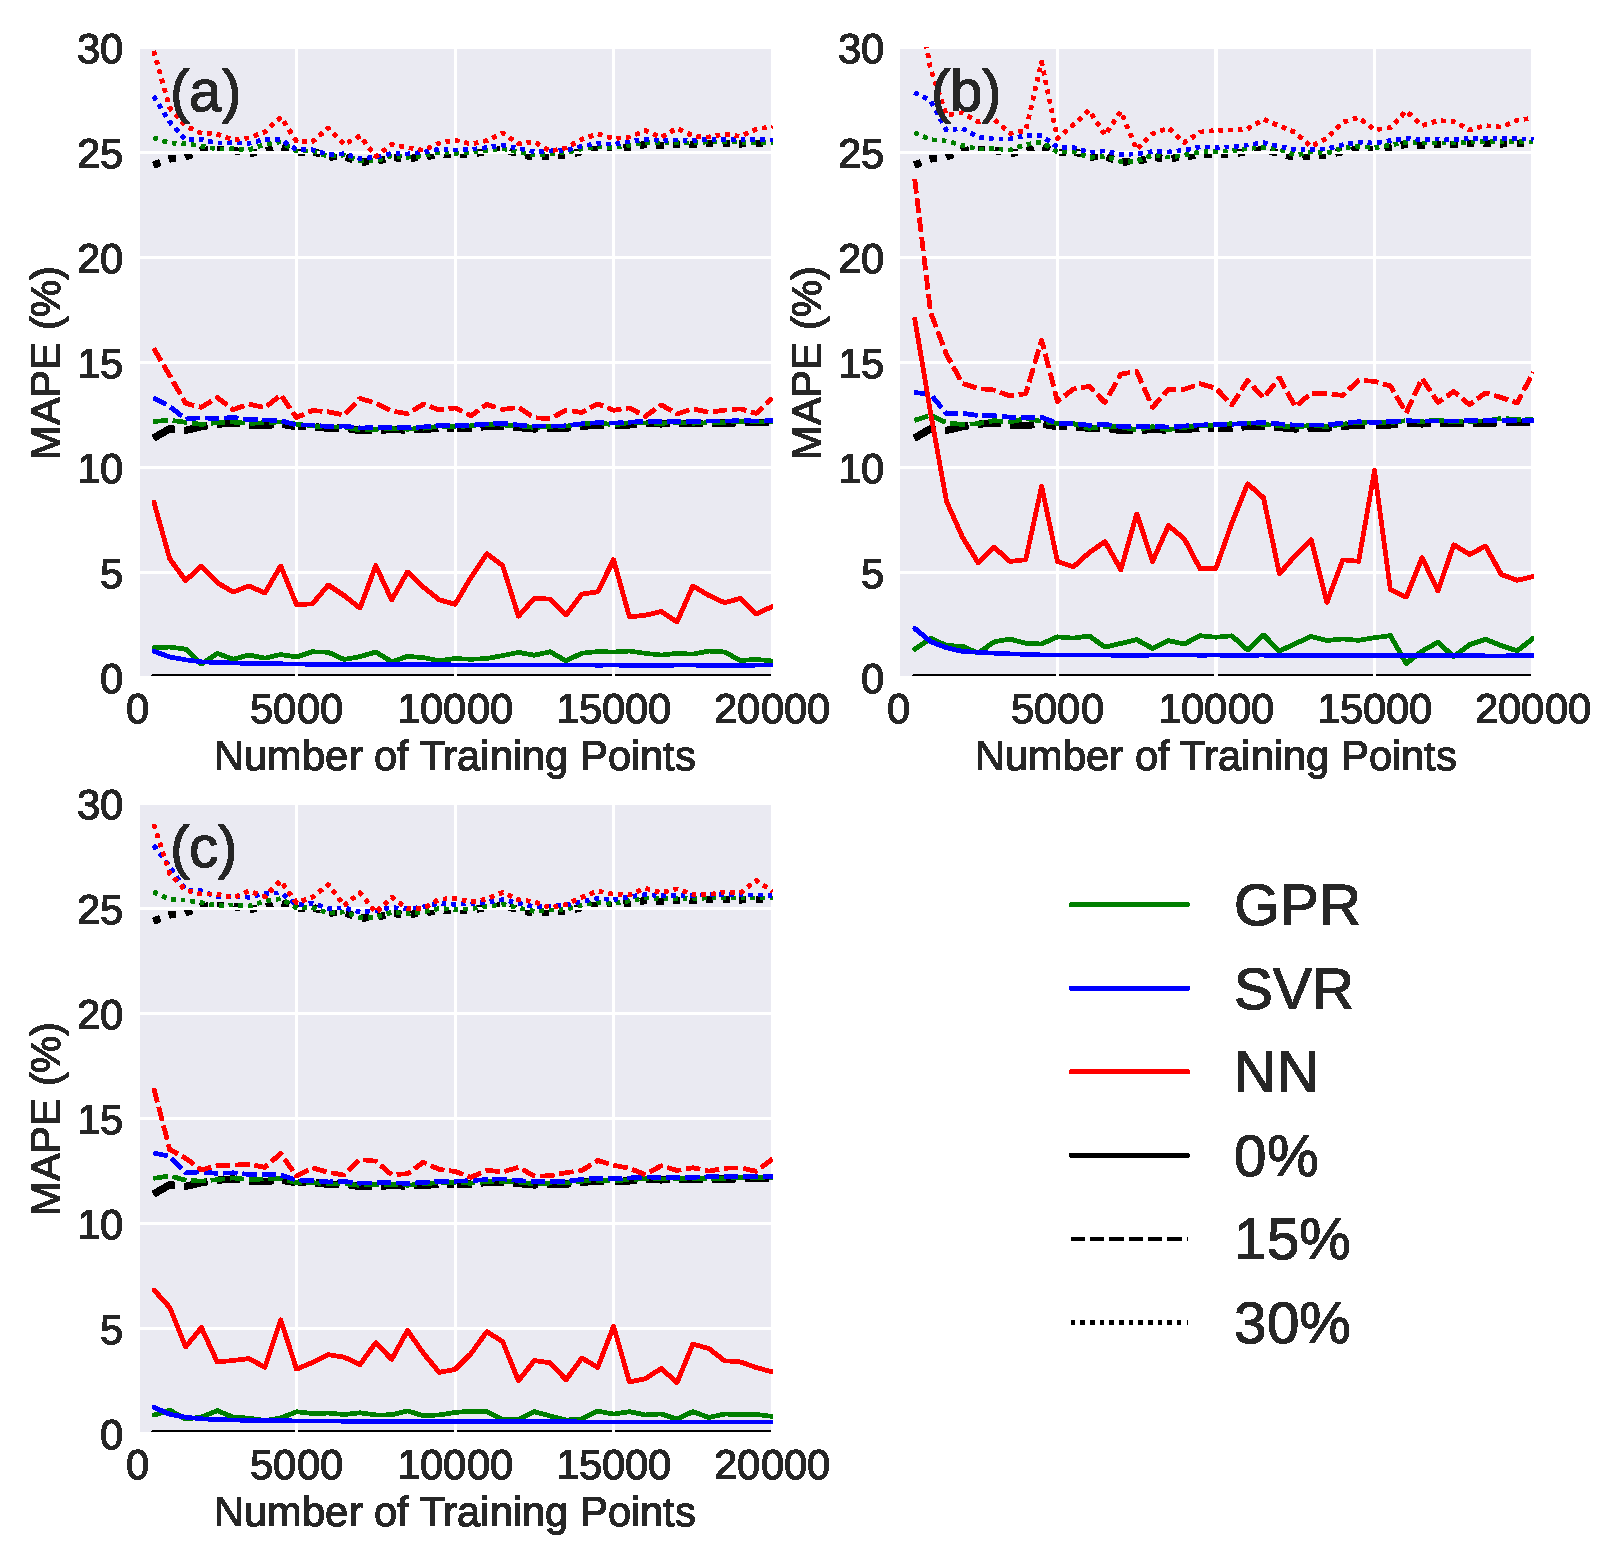
\includegraphics[width=0.75\linewidth]{planning/images/paper1/test_mape_3levels.eps}
	\caption{MAPE versus number of training points from ML model predictions for (a) max proton energy, (b) total proton energy, (c) average proton energy and noisy testing data. Each panel shows results from (solid) 0\%, (dashed) 15\% and (dotted) 30\% added noise in the data. Black lines with different line types indicate the MAPE between the noisy and noiseless data. Because we only compare ML models to noisy data in this figure, these black lines indicate the best that any ML model could conceivably do. Figure and caption taken from Figure 3 of Desai et al. \cite{Desai_2024_CPP}.}
	\label{fig:mape_3levels}
\end{figure}

Then, we kept the number of data points fixed at 2,000 and varied the noise level from 0 to 30\% to make a similar analysis in \autoref{fig:mape_noise}. These plots show how the \gls{NN} model doesn't do well without any added noise. In addition to the noisy test data (solid line), the error on the same data without noise was also plotted as a dashed line. One interesting feature about this plot is that the \gls{NN} model's error does not increase significantly as the noise level increases. 

\begin{figure}
	\centering 
	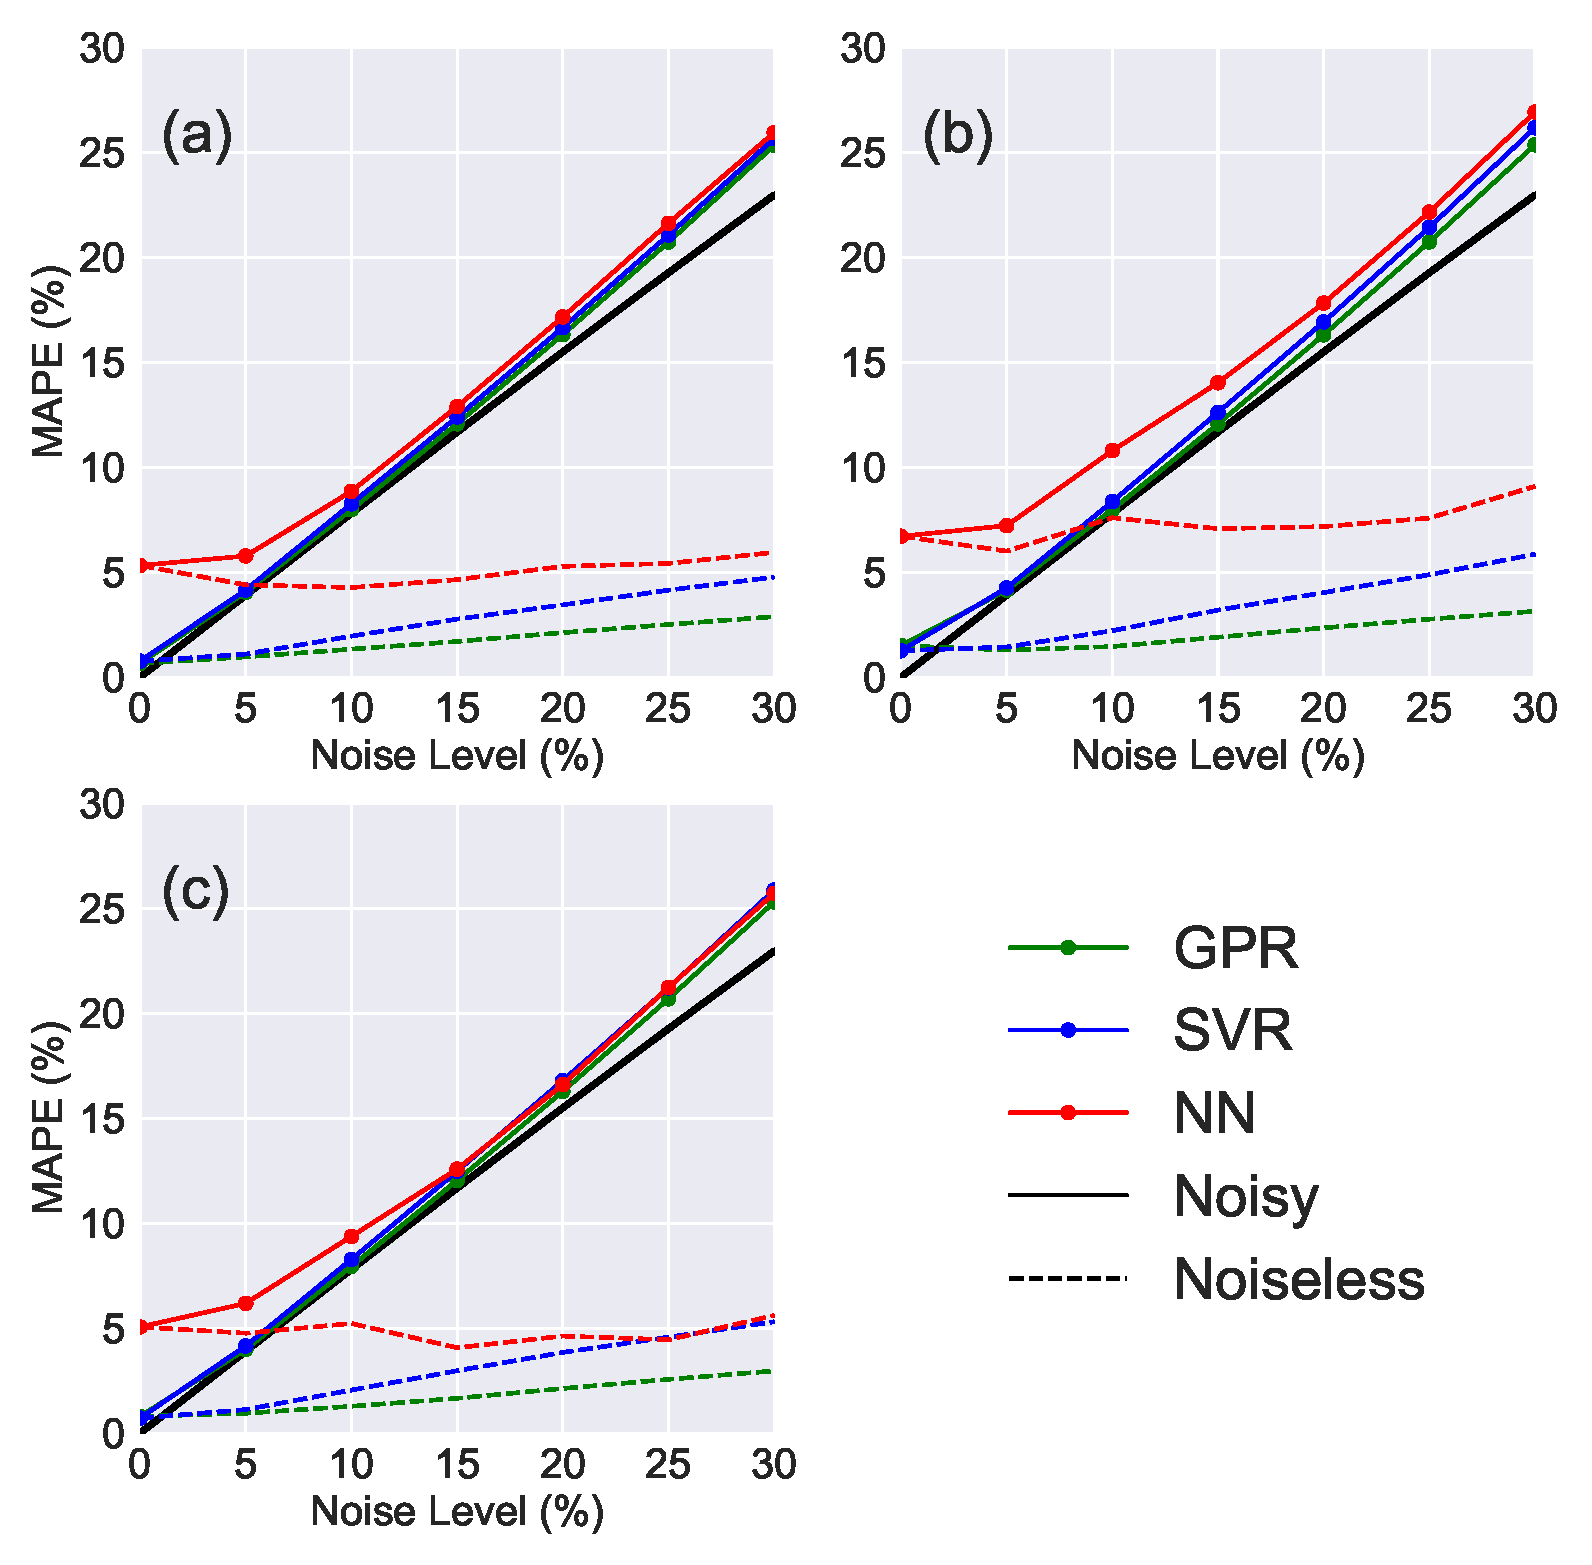
\includegraphics[width=0.75\linewidth]{planning/images/paper1/test_mape_points=2.0k.eps}
	\caption{Solid lines show the typical MAPE in (a) maximum proton energy, (b) total proton energy, and (c) average proton energy when the models (which were trained on 2000 synthetic data points with noise) are evaluated on data with different levels of noise. Dashed lines show the typical error when those same ML models are evaluated on noiseless test data. Black solid lines indicate the MAPE between the noisy and noiseless data. Figure and caption taken from Figure 4 of Desai et al. \cite{Desai_2024_CPP}.}
	\label{fig:mape_noise}
\end{figure}

Next, we compared the execution time of the different \gls{ML} models and found that the \gls{SVR} runs the fastest, the \gls{GPR} runs the slowest, and the \gls{NN} runs at a speed somewhere in between. The \gls{GPR} scales roughly as $\mathcal{O}(N^3)$ \cite{Wang_2019_GPytorch} which can be contrasted with the \gls{NN}s $\mathcal{O}(N)$. In terms of GPU memory utilized, the \gls{GPR} used 14 GB, whereas the \gls{SVR} and \gls{NN} used between 1 and 2 GB. Due to the unfavorable $\mathcal{O}(N^2)$ memory scaling of the \gls{GPR} \cite{Wang_2019_GPytorch}, larger datasets than 40,000 points were practically infeasible with our implementation.

\begin{figure}
	\centering 
	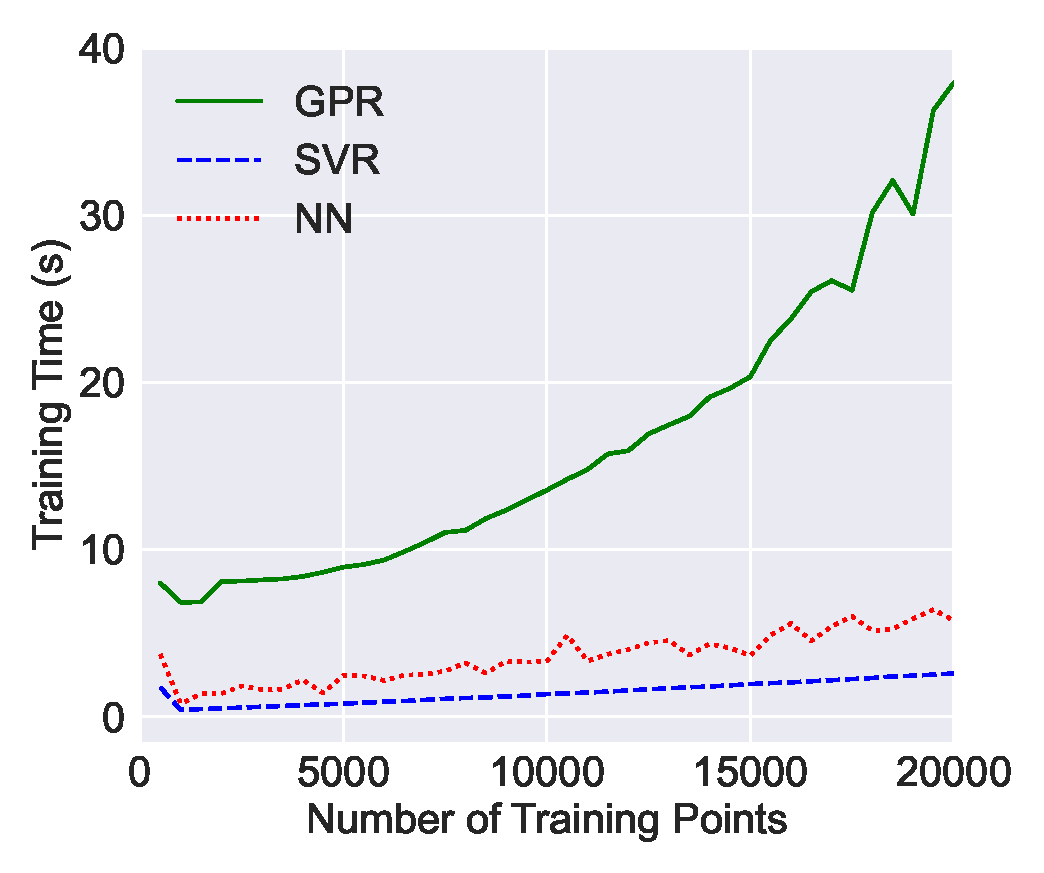
\includegraphics[width=0.6\linewidth]{planning/images/paper1/time.eps}
	\caption{The execution time of the different ML models averaged across noise levels in computing the maximum, total, and average proton energies. Figure and caption taken from Figure 5 of Desai et al. \cite{Desai_2024_CPP}.}
	\label{fig:execution_time}
\end{figure}

\subsection{Optimization Task}
\begin{figure}
	\centering 
	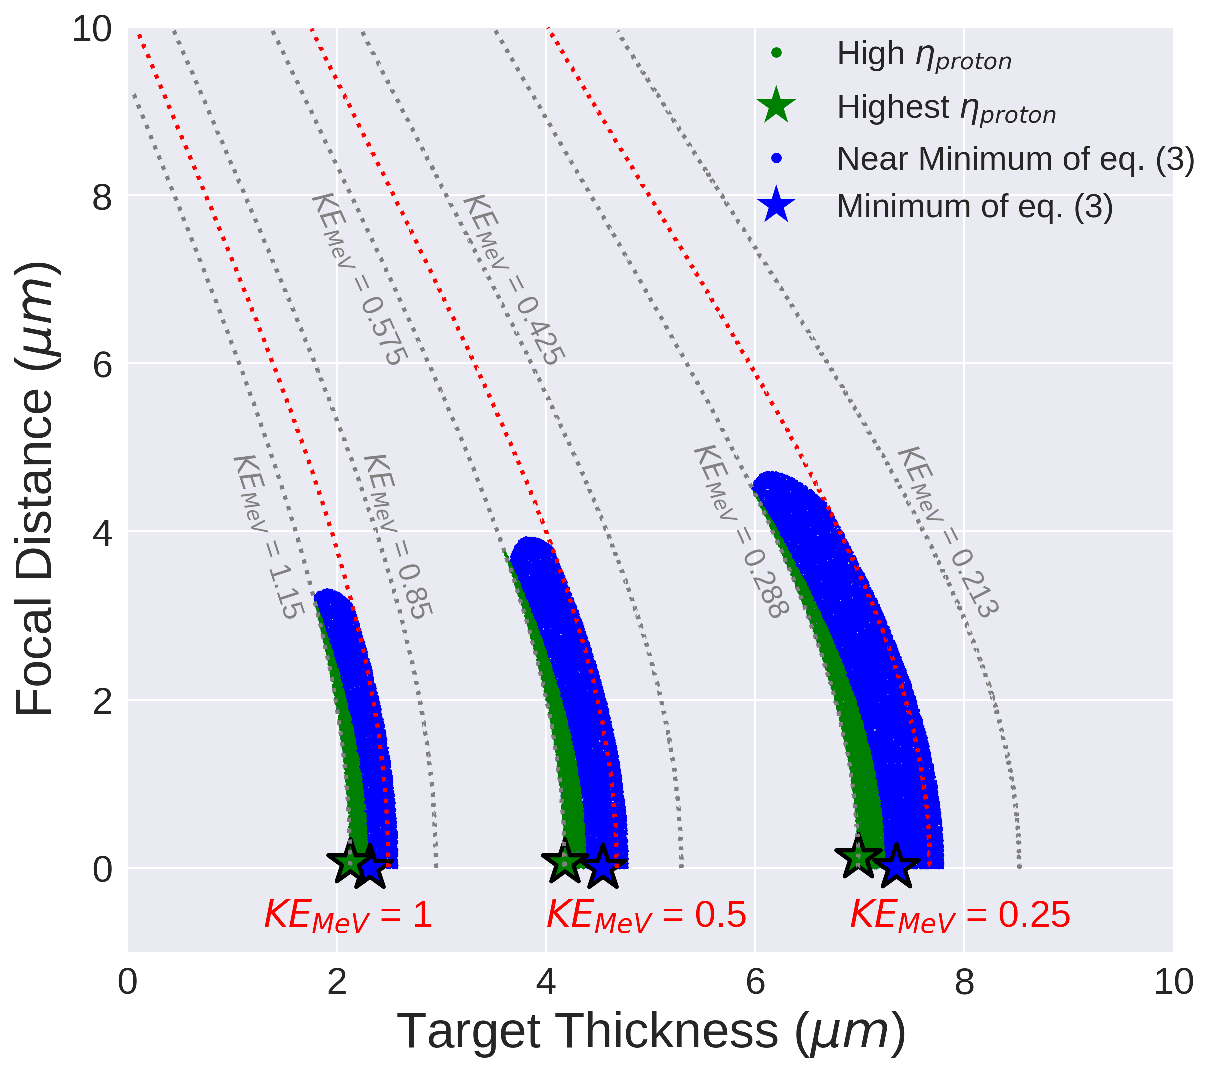
\includegraphics[width=0.65\linewidth]{planning/images/paper1/fuchs_optim.pdf}
	\caption{Parameters that produce maximum proton energy cutoffs in three different desired ranges: 1.0~MeV, 0.5~MeV and 0.25~MeV. Combinations of thickness and focal distance that produce these energy cutoffs (irrespective of the laser to proton conversion efficiency) are shown with dotted red lines. With each red line we also show with dotted gray lines the thicknesses and focal distances that produce proton energy cutoffs that are +15\% or -15\% of the cutoff goal. Green shaded areas show regions where the laser to proton conversion efficiency is high (i.e. within 5\% of the optimal value). A green star shows the ideal conditions for maximizing the proton conversion efficiency. The blue region corresponds to using all the terms in \autoref{eq:fuchsv1_function} and the blue star indicates the ideal conditions according to that minimization scheme. Figure and caption taken from Figure 6 of Desai et al. \cite{Desai_2024_CPP}.}
	\label{fig:banana}
\end{figure}

We highlighted a useful application of these models by determining a set of inputs that would produce a proton energy spectrum up to a specified maximum energy with a relatively high number of protons in that range as well. We characterize the balance of these two quantities, the maximum cutoff energy $KE_\text{c}$ ($E_\text{max}$) and the laser to proton conversion efficiency $\eta_\text{p}$ ($E_\text{tot} / E_\text{laser}$), as 

\begin{equation}
	f(KE_{\rm c},\eta_{p}) = \frac{|KE_{\rm c} - KE_{\rm c,goal}|}{KE_{\rm c, goal}} + \frac{C}{\eta_{p}} + g( KE_{\rm c},KE_{\rm c,goal})  \\ \label{eq:fuchsv1_function}
\end{equation}
where $C$ is a parameter that can influence the strength of $\eta_\text{p}$ relative to $KE_\text{c}$. These features can seen in \autoref{fig:banana} where three different energy cutoffs were chosen to optimize towards: 1, 0.5, and 0.25 MeV. The green region focuses on regions of the parameter space that closely match the given cutoff, while the blue region additionally factors in $\eta_\text{p}$. For practical reasons, we impose a penalty term $g(KE_\text{c}, KE_\text{c, goal})$ that prevents choosing points that have $KE_\text{c}$ more than 15\% away from the specified cutoff. These plots are generated from the Fuchs et al. model with 0 added noise, so they should be regarded as the ideal results that can be compared with the \gls{ML} models.

\begin{figure}
	\centering 
	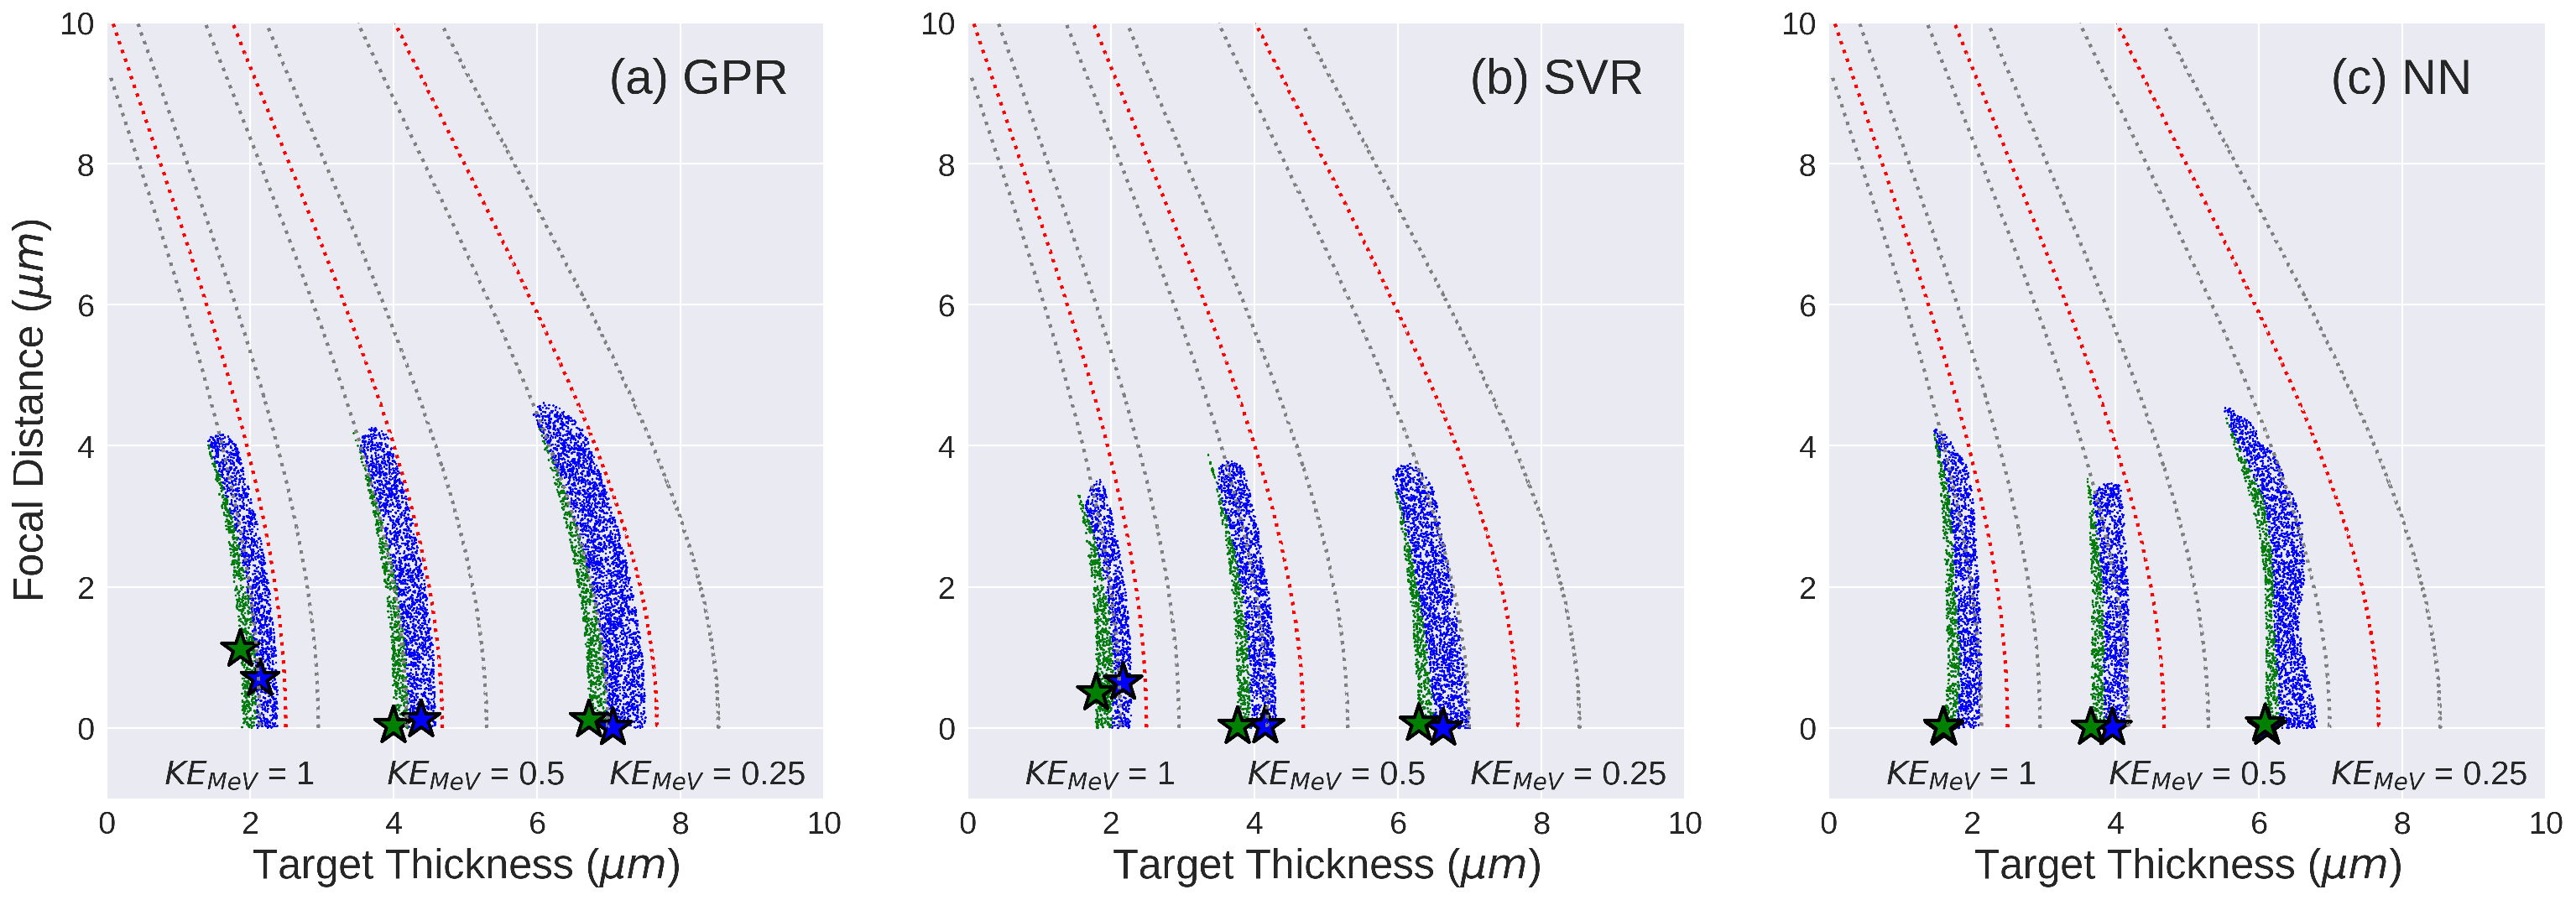
\includegraphics[width=0.95\linewidth]{planning/images/paper1/model_optim_noise=30_pts=2000.pdf}
	\caption{Parameters that produce maximum proton energy cutoffs according to three trained ML Models on 2,000 data points with 30\% added noise: (a) GPR, (b) SVR, (c) NN compared against the red and gray lines plotted in \autoref{fig:banana}. The green and blue shaded regions are scatter plots of a subset of evaluated points that fall within 5\% of the model's predicted optimum according to the same criteria in \autoref{fig:banana}. Figure and caption taken from Figure 7 of Desai et al. \cite{Desai_2024_CPP}.}
	\label{fig:banana3}
\end{figure}

We generated the same plots\footnote{These plots are colloquially referred to as \emph{banana} plots in my research group due to their shape.} as \autoref{fig:banana} with trained \gls{ML} models on 2,000 training data points with 30\% added noise which can be seen in \autoref{fig:banana3}. These results show the \gls{GPR} closely matching \autoref{fig:banana} and the \gls{SVR} performing similarly well. Meanwhile, the \gls{NN}'s predicted point often fall outside the 15\% cutoff boundary, which is not surprising due to its lower accuracy from the preceding analysis in \autoref{fig:mape_noise}. 

\section{Second Analysis} \label{sec:second_analysis}

In this section, my work from \autoref{sec:first_analysis} was expanded upon and written into a manuscript that is currently under consideration at \emph{APL Machine Learning}. This work was originally assigned to (then) undergraduate student Jack Felice as a similar, but complementary project to what I primarily worked on. Jack did the bulk of the work in this project and borrowed help from me as needed. When Jack left for graduate school at the University of Maryland, I spent a few months organizing his work, contributing to the text of the paper, and creating polished figures. The co-authors from this work are largely the same as the previous work, but additionally include fellow graduate student Nathaniel Tamminga for his discussion on the constrained data campaign. This work was also modeled on the \gls{WP-ELL} laser system.

\subsection{Methods}
In \autoref{sec:first_analysis}, we tried to address training a model on only 20,000 data points. Furthermore, this model was relatively simple -- a regression algorithm could fit the model quite accurately with only a few thousand points. Also, we found that the \gls{NN} model performed poorly due to lack of model complexity and too few data points. A real experimental dataset would be much more complex and thus require more data to understand its underlying trends. As a result, our second project added complexity in the form of pre-expansion of the target explained in \autoref{sec:fuchsv2}. 

From this new modified model, we generated a training dataset of 1,525,000 points by sampling from a uniform grid of points in a 4D parameter space. The three inputs from \autoref{sec:first_analysis} are the same (except we reduced the maximum of the target thickness to $\SI{5}{\micro \meter}$). This grid included thicknesses in steps of $\SI{0.5}{\micro \meter}$, focal positions in steps of $\SI{1}{\micro \meter}$ and intensities in steps of $\SI{1.8e17}{\watt \per \centi \meter \squared}$. The relevant quantity to control the extent of the pre-plasma is the contrast $\kappa$ which was varied in steps of $1.8 \times 10^{-8}$. In \autoref{fig:density_profile}, the effect of the prepulse can be seen modifying the density profile of the target ($t_0 = 60$ ps was used in this work). The 250,000 point testing dataset was generated from the same intervals as the training set, but without noise and on a grid of points (instead of random sampling throughout the interval).

We used the same outputs as before: $E_\text{max}$, $E_\text{tot}$, and $E_\text{avg}$. Since the new contrast parameter can make the proton energies get arbitrarily low, we set a floor to these outputs energies of 1 keV, 1 nJ, and 1 keV respectively. This was motivated by the finite energy resolution of ion energy detectors and preventing the \gls{MAPE} metric from getting a division by zero error. Additionally, the acceleration time multiplier (see \autoref{eq:fuchs_multiplier}) was increased to 25 to balance out the lower predicted proton energies from the new physics model's larger effective thickness (\autoref{eq:d_eff}). The features of this new model can be seen in \autoref{fig:density_profile} which highlight the characteristic \emph{dip} in the proton energy at peak focus obtained from Morrison et al. \cite{Morrison_2018_NJoP}.

We used a \gls{NN} model like the previous work in \autoref{sec:first_analysis}, but modified the other two models. The \gls{SVR} was not able to handle more than a few hundred thousand data points and for this reason, it was not used. Instead, we used the more elementary \gls{POLY} due to its simplicity which can be used as a baseline model without \gls{GPU} accelerated computations. The \gls{POLY} model could fit the data in \autoref{sec:first_analysis} accurately, but it does not work well with the added complexity in the new model (which will be seen later). Then, we replaced the exact \gls{GPR} with the \gls{SVGP} (see \cite{Hensman_2014_SVGP}) which assumes a variational distribution over some amount of inducing points, restricting the training data to a representative subset. This allows the \gls{SVGP} to be trained on data sets of order one million points in mini-batches just like the \gls{NN}. Like before, we summarize the hyperparameters in \autoref{tab:hps2}.  Finally, we replaced the standard z-score normalization with min-max scaling -- a linear scaling that scales the minimum value of a particular data column to be 0 and the maximum value to be 1. Min-max scaling was chosen to better represent the nature of parameter selection: uniform sampling between some minimum and maximum value.

\begin{table}
	\centering
    \begin{tabular}{|c|c|c|c|}
	\hline
	Model & Parameters & RMSE & Time (min)   \\
	\hline
	POLY & deg=7, $\alpha=10^{-3}$  & 0.033 & 0.883 \\ 
	\hline
	SVGP & IP=2000, LF=8, LR=$10^{-2}$  & 0.018 & 34.66 \\ 
	\hline
	NN  & BS=$2^{13}$, $\gamma=0.90$, P=10 & &\\
	& LR=$10^{-2}$, 12x64  & 0.013 & 4.93 \\ 
	\hline
\end{tabular}
	\caption{Optimal hyper-parameters including the root mean square error (RMSE) and mean fit time, determined from a grid search of hyperparameters for the NN, POLY, and SVGP. For the NN, the batch size (BS), learning rate decay ($\gamma$), patience (P), learning rate (LR), and architectures (layers x neurons per layer) were changed throughout the scans. For the POLY, the regularization parameter ($\alpha$) and degree (deg) were varied. For the SVGP, the number of inducing points (IP), latent functions (LF), and learning rate (LR) were changed throughout the scans.}
	\label{tab:hps2}
\end{table}

\subsection{Results}

In \autoref{fig:train_time_accuracy}a, the \gls{MAPE} is calculated for each of the three \gls{ML} models with a variable number of training data points from a dataset with 10\% added noise. The \gls{MAPE} is evaluated on the fixed size testing dataset of 250,000 points. With the \gls{NN} and \gls{SVGP} models, 20\% of the training set was reserved for validation so model training could stop early if the validation error stopped decreasing. Here, we can clearly see that the \gls{NN} and \gls{SVGP} have a significantly lower percentage error than the \gls{POLY}. Additionally, \autoref{fig:train_time_accuracy}b shows that the \gls{SVGP} takes significantly longer than the \gls{NN} to train which in turn takes significantly longer than the \gls{POLY} (note the logarithmic scale).

\begin{figure}
	\centering
	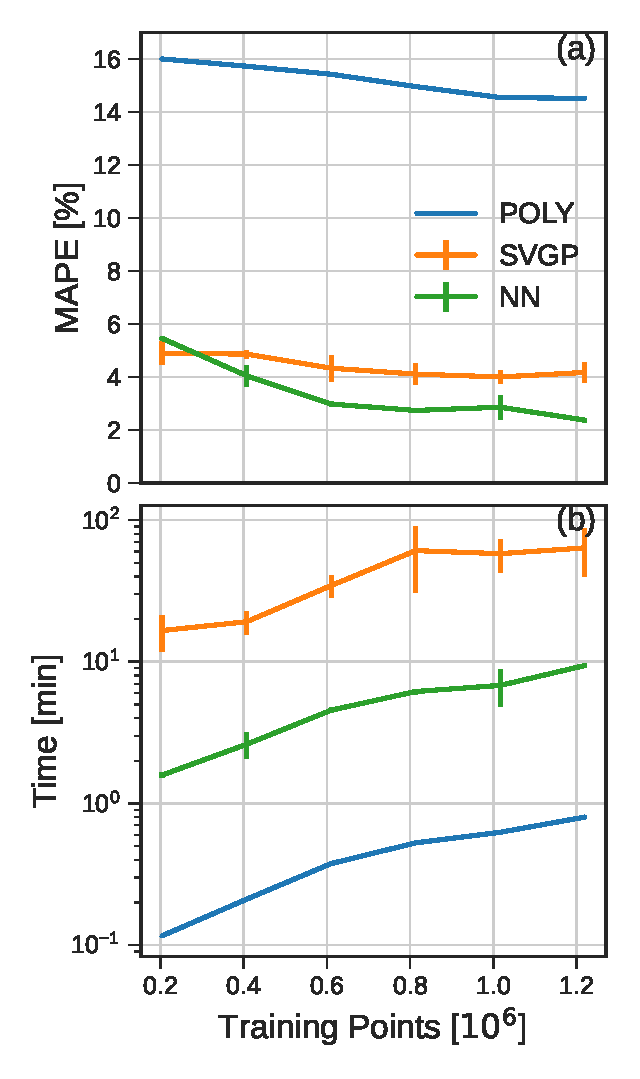
\includegraphics[width=3.5in]{planning/images/paper2/fig4.eps}
	\caption{Model training results using data with 10\% added noise. Testing MAPE (a) is plotted for the three ML models against the number of training points and averaged between results for maximum, average, and total proton energy. The training time (b) of the ML models in minutes is plotted on a logarithmic scale. The vertical bars are standard deviations computed from running the training splits 3 times with different seeds to control the data splitting and random parameter initialization of the NN and SVGP models.}
	\label{fig:train_time_accuracy}
\end{figure}

Then, like in \autoref{sec:first_analysis}, we analyzed the effect of changing the noise level in \autoref{fig:noise_accuracy}. We can see that the \gls{POLY} again has the worst accuracy which does not change with the noise level. While the \gls{SVGP} and \gls{NN} are more accurate, the \gls{SVGP} seems to perform worse at a higher noise level.

\begin{figure}
	\centering
	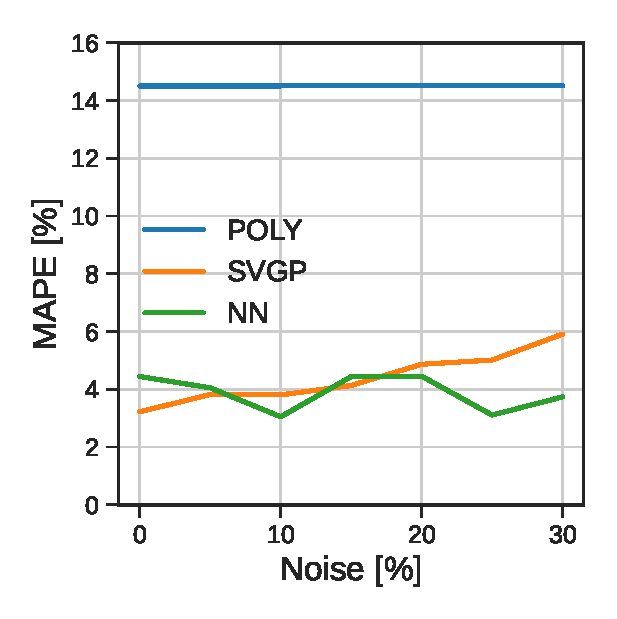
\includegraphics[width=3.5in]{planning/images/paper2/fig5.eps}
	\caption{Testing MAPE is plotted against different levels of gaussian noise using the full training dataset for the three models with the three output energy results averaged.}
	\label{fig:noise_accuracy}
\end{figure}

\subsection{Optimization Task}
Similar to \autoref{sec:first_analysis}, we came up with an optimization task to demonstrate the effectiveness of the models. This time, we used a slightly different objective function 

\begin{equation}
	f(KE_{\rm c},\eta_{p}) = \frac{|KE_{\rm c} - KE_{\rm c,goal}|}{1 \text{MeV}} \beta - 100 \eta_{p} (1-\beta) \label{eq:obj_function_v2}
\end{equation}
which can be contrasted to \autoref{eq:fuchsv1_function}. One notable difference is the subtraction of the conversion efficiency $\eta_\text{p}$ instead of adding $1 / \eta_\text{p}$. This allows us to control the relative strength of the two terms through a quantity $\beta$ that varies from 0 to 1. \autoref{fig:energy_efficiency} shows the distribution of $\text{KE}_\text{c}$ (i.e. $E_\text{max}$) and $\eta_\text{p}$ (i.e. $E_\text{tot} / E_\text{laser}$) as a function of target thickness and focal position when fixing the intensity and contrast to the maximum and minimum within their respective ranges.

\begin{figure}
	\centering
	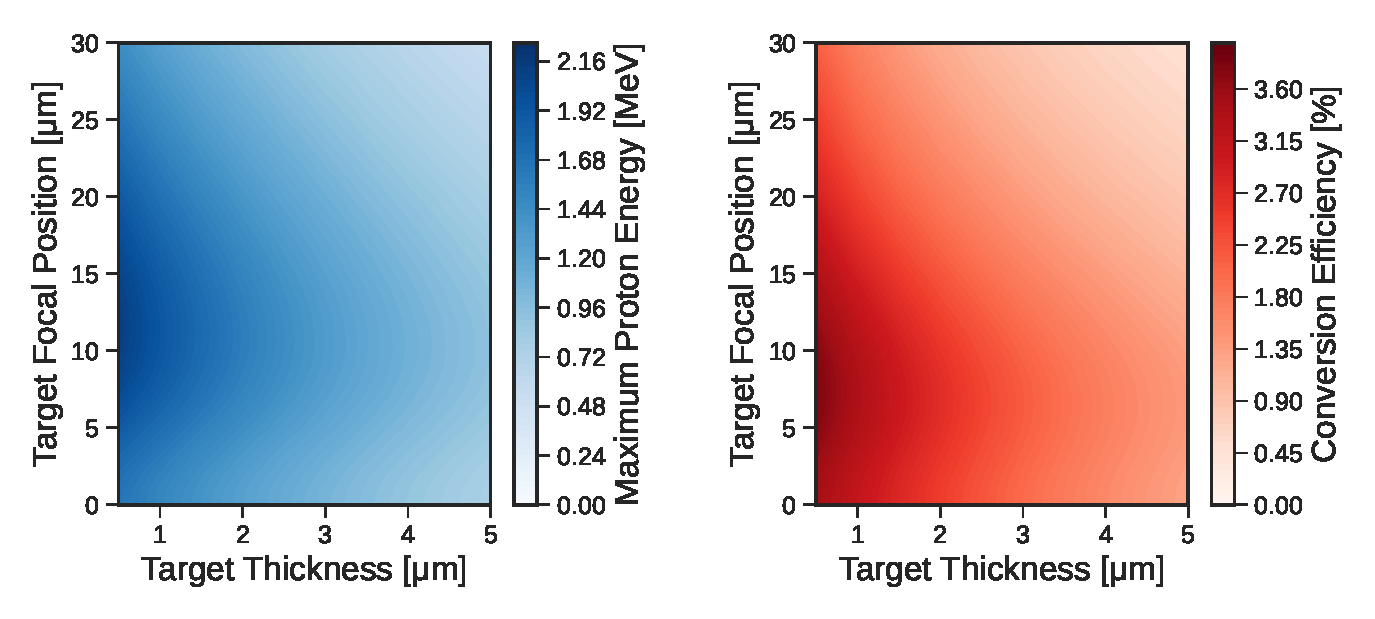
\includegraphics[width=6in]{planning/images/paper2/fig6.eps}
	\caption{Colormaps in the 2D parameter space of target thickness and target focal position that display (left panel) the maximum proton energy (i.e. energy cutoff $KE_{\rm c}$) and (right panel) laser to proton energy conversion efficiency $\eta_{p}$ as calculated from the modified Fuchs et al model. These plots were generated assuming 14.14~mJ of laser energy and a pre-pulse contrast of $10^{-7}$.}
	\label{fig:energy_efficiency}
\end{figure}

For our optimization task, we used the models trained on 30\% added noise to sample a set of points which fixes the laser energy at 14.14mJ (by assuming $I_0 = 10^{19} \text{W cm}^{-2}$) and the contrast to $\kappa = 10^{-7}$, but varied the target thickness and focal distance. The thickness and focal distance were stepped in $\SI{0.1}{\micro \meter}$ increments to generate a 2D grid of 13,846 points to evaluate the trained models on. Notably, the step sizes are 5-10 times smaller than what was used in the dataset generation so that the models will be forced to interpolate between points not originally seen by the trained models. 

The optimum conditions that minimize \autoref{eq:obj_function_v2} are indicated with a star in \autoref{fig:obn_fn_model} for a range of $\beta$ values. In this analysis, the goal cutoff is fixed at $\text{KE}_\text{c, goal} = 1$ MeV, but this approach can easily be generalized to a different value. The upper panels of \autoref{fig:obn_fn_model} are the results from the analytic model (noiseless) and should be regarded as the true distribution of \autoref{eq:obj_function_v2}. The optima of these panels are indicated with a white star. The other rows show the estimated distribution according to the three \gls{ML} models and have predicted optima shown with a cyan star. For comparison, the white star from the analytic model is overlayed on each panel.

\begin{figure}
	\centering
	\includegraphics[width=6.5in]{planning/images/paper2/fig7.eps}
	\vspace{-0.4cm}
	\caption{Colormaps that show estimates of \autoref{eq:obj_function_v2} assuming $KE_{\rm c,goal} = 1$~MeV for the three ML models (NN, POLY and SVGP) and the modified Fuchs et al. model dataset with no added noise (FUCHS). The modified Fuchs et al. model with 30\% added noise was used to produce the training data for the ML models. For each $\beta$ value (i.e. each column), the same color levels are used in order to facilitate comparison between the models. A cyan colored star is placed at the location where each ML model predicts a minimum value for \autoref{eq:obj_function_v2} which can be compared to the analytic model prediction indicated by a white star.}
	\label{fig:obn_fn_model}
\end{figure}

In \autoref{fig:obn_fn_model}, one can see that for $\beta = 0.25$, the best (i.e. globally minimum) region is at 0.5~$\mu$m thickness and 10~$\mu$m focal position, which correspond to regions with higher $\eta_{p}$. The \gls{POLY} and \gls{SVGP} models predict the optimal conditions to be at a focal position of $\sim15~\mu$m, in contrast to the \gls{NN} prediction of $\sim11~\mu$m. In this case, the \gls{NN} more closely matches the true optimum. For high values of $\beta$, the best region is a curve composed of points that closely match $KE_{\rm c}$ to $KE_{\rm c,goal}$. Using the highest value of $\beta = 1$, we see that while the \gls{NN} looks much less smooth, it fits the overall shape of the underlying Fuchs model better than the other two methods.

The features of \autoref{fig:obn_fn_model} are quantified in \autoref{tab:opt_results}. We can assess the accuracy of the optimal conditions by taking the Euclidean distance in the focal position - target thickness space between the true optimum conditions and the \gls{ML} predictions. This distance, termed $\Delta_\text{opt}$, shows that (with the exception of $\beta=1$), the \gls{NN} predicted optimum is closer to the true model than the \gls{SVGP} or \gls{POLY}. To assess accuracy in the colormap as a whole, we can take the \gls{RMSE} between the analytic model and the ML model's colormap values which clearly show lower error for the \gls{NN} in comparison to the \gls{SVGP} and \gls{POLY}.

\begin{table}
	\centering
	\begin{tabular}{|c||c|ccccc|}
		\hline
		&$\beta$   & 0        & 0.25     & 0.5      & 0.75     & 1        \\ 
		\hline
		& POLY & 0.329   & 0.223  & 0.121   & 0.057 & 0.124  \\
		RMSE & SVGP & 0.143  & 0.096 & 0.062 & 0.065 & 0.101  \\
		&NN   & 0.065 & 0.052 & 0.042 & 0.038 & 0.042 \\
		\hline 
		& POLY & 4.5 & 5.5  & 7.5     & 9.489  & 2.121 \\
		$\Delta_\text{opt}$ [$\mu$m] &SVGP & 3.5 & 4.5  & 5.601 & 4.148  & 4.144 \\
		&NN   & 0.4 & 1.2  & 3.1     & 0.825 & 4.717 \\
		\hline
	\end{tabular}
	\caption{Comparison metrics evaluated from \autoref{fig:obn_fn_model}. The RMSE row shows the root mean squared error between the colormap values of the ML models and the analytic model for each value of $\beta$. The $\Delta_\text{opt}$ row calculates the Euclidean distance between the predicted optimum and true optimum (i.e. distance in $\mu$m between the cyan and white stars in \autoref{fig:obn_fn_model}).}
	\label{tab:opt_results}
\end{table}
 
\subsection{Constrained Data Campaign}

Earlier, we describe how synthetic data was generated using a uniform grid in multiple dimensions of laser and target parameters. The primary training set data for the ML models discussed in the main body of the paper was obtained with this scheme. From an experimental point of view, this approach is not very realistic because a real laser system will scan through the laser and target parameters in a very specific way with specific choices. For example, certain parameters could vary first while keeping other parameters constant, and then the opposite could happen to explore a different parameters. How do these choices affect the accuracy of \gls{ML} models trained on this data? This is a question that we cannot yet answer conclusively, but we include an investigation into two realistic parameter scans (a.k.a. ``campaigns'') that are used to train \gls{ML} models instead of the uniform grid approach.

As highlighted in \autoref{fig:zigzag}, there were two experimental ``campaigns" used to produce synthetic data -- one where thickness, focal depth and laser energy were varied, and another where thickness, laser energy and pre-pulse contrast were varied between. All the synthetic data from the two campaigns were used to train \gls{ML} models. In this way, our training set includes variation in four different input parameters.

The first campaign was generated by stepping through thickness-intensity coordinates, incrementing the focal distance by \SI{3}{\micro \meter} and the thickness by \SI{0.05}{\micro \meter}, performing a full scan of focal depth values at \SI{0.5}{\micro \meter} and every integer value until \SI{5.0}{\micro \meter}.  At each point along the thickness-intensity curve, a full sweep of intensity was performed.  Since, in a real experiment, the intensity can be controlled by varying a polarizing wave plate, the synthetic data set for this investigation varied the intensity by multiplying the maximum intensity value ($10^{19}$~\unit{W . cm^{-2}}) by the cosine-squared of an angle (which could be a polarizing waveplate), which was varied from $0^{\circ}$ to $70^{\circ}$ and back over the course of an intensity sweep.  The resulting sweep is depicted in \autoref{fig:zigzag}a, creating a set of 1.15 million data points.  

The second campaign was generated in a similar manner, but because, in a real experiment, neither main pulse nor pre-pulse laser intensity have an appreciable effect on target stability, both were able to be varied simultaneously.  As such, the data set was generated by incrementing thickness by \SI{0.05}{\micro \meter} from $0.5$ to $5.0$ \unit{\micro \meter}, taking a full scan of both main pulse intensity and contrast at every thickness value.  The pre-pulse contrast was varied in the same manner as the main pulse intensity, so the contrast was varied according to a cosine-squared function of another angle.  The resulting data are depicted in \autoref{fig:zigzag}b, with an overall size of 1.27 million data points.

\begin{figure}
	\centering
	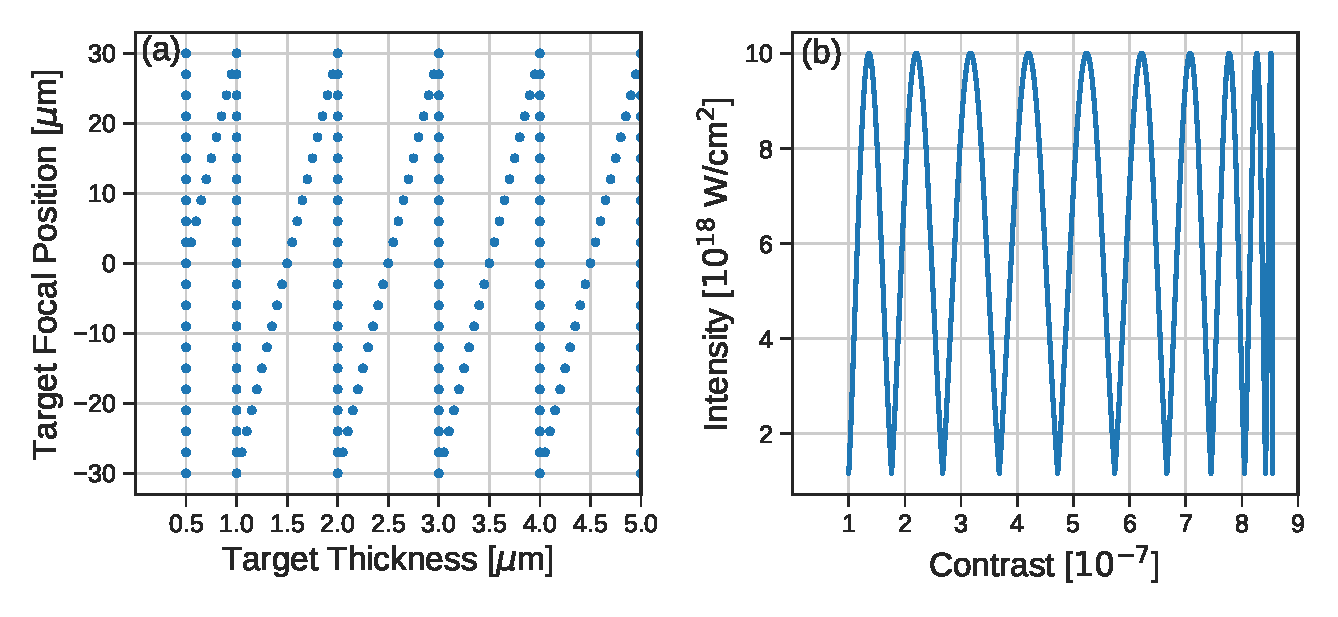
\includegraphics[width=6.5in]{planning/images/paper2/fig10.eps}
	\caption{Synthetic data was generated in one of two ``campaigns''. In (a) campaign 1, the target focus and thickness is varied in discrete steps and each blue dot varies the laser energy from minimum to maximum. In (b) campaign 2, the depicted intensity and contrast looping is performed for discrete steps in target thickness from $0.5~\mu$m to $5\mu$m}
	\label{fig:zigzag}
\end{figure}

In both campaigns, choices about how many increments to make for different parameters were influenced by a constraint that each campaign last no more than about an hour on a 1~kHz repetition rate laser system. Both campaigns assumed 10\% added gaussian noise, following the same prescription used in both \autoref{sec:first_analysis} and \autoref{sec:second_analysis}. The combined training set, which includes data from both campaigns, has a total size of 2.42 million points. To better compare with earlier results shown in \autoref{fig:train_time_accuracy}a in which the ML models were trained with different numbers of training points, we randomly sampled from this data set to utilize a similar number of points. To test the accuracy of the trained \gls{ML} mdoels, we use the same testing set utilized in \autoref{fig:train_time_accuracy}a, which did not include any noise. Our results are shown in \autoref{fig:split_accuracy}. 

\autoref{fig:split_accuracy} shows that, overall, the \gls{NN} and \gls{SVGP} models have a much higher \gls{MAPE} than was seen earlier in \autoref{fig:train_time_accuracy}a. Also, a third order polynomial fits the data set almost as well as the NN and SVGP which indicates that NN and SVGP models are not able to fit the underlying model very well when trained on data split into the two campaigns we described. A possible improvement could be an experimental design where both the target focal position and the pre-pulse contrast are varied simultaneously, rather than keeping the contrast fixed and varying the target focal position (first campaign), and then varying the contrast while keeping the target focal position fixed (second campaign). But varying as many as four parameters simultaneously creates its own challenges for exploring a large parameter space in a relatively short amount of time ($\sim$~1-2~hours).

\begin{figure}
	\centering
	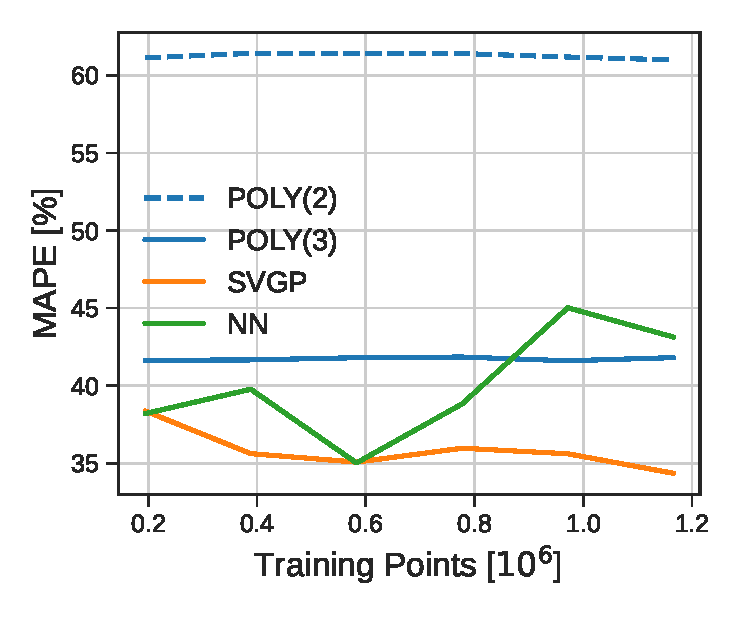
\includegraphics[width=4in]{planning/images/paper2/fig11.eps}
	\caption{Testing set MAPE evaluated on several ML models trained on data combined from two separate campaigns shown in \autoref{fig:zigzag}. The dashed line differs from the solid blue line in the polynomial degree.} The different data splits are chosen to be approximately the same as what was shown in \autoref{fig:train_time_accuracy}.
	\label{fig:split_accuracy}
\end{figure}

\section{Conclusion} 

In \autoref{sec:fuchs_model}, we reviewed the physics of the isothermal expansion model for which the Fuchs et al. model is based upon. Then, we showed the modifications that we made to the model to better fit data at the Extreme Light Laboratory at the Wright-Patterson Air Force Base and account for pre-expansion of the target. From this modified model, we were well equipped to construct a synthetic dataset that could have multiple inputs/outputs and added noise.

Then, in \autoref{sec:first_analysis}, we summarized our first machine learning effort which analyzed a 25,000 point dataset with three machine learning methods: gaussian process regression, neural networks, and support vector regression. In this work, we generally found that the neural network model was the least accurate and had the worst performance on our optimization task. This was not that surprising because neural networks generally only work well for complex datasets. The gaussian process regression and support vector regression were both similarly accurate; in part, this was due to the relatively simple physics model we used. However, the gaussian process consumed a lot of memory and would be unsuitable for larger datasets. 

Next, in \autoref{sec:second_analysis}, we described the second machine learning effort which expanded upon the first by using a dataset of over 1 million points. Here, we also used a more complex model that accounted for an additional input (pre-pulse contrast). We did a similar analyis and found that the added complexity actually made the neural network model a more favorable choice. We used a different implementation of the gaussian process which was capable of handling the million point dataset and achieved good accuracy, but still suffered from long run times. The added complexity also made it difficult for the simpler polynomial model to fit the data.

Throughout this chapter, we explored a novel idea in the field of plasma physics: generating a synthetic dataset based on modifications of established physical models to provide machine learning insights. Our model could, in principle, further be improved to take into account other phenomena that a 1D model could not capture like the shape of the target or the laser angle of incidence. Even though the model may not match up exactly to experiment, it would have the desired trends expected from a real experiment which can at least give us insights into how a hypothetical machine learning framework might operate. By offering the code and synthetic datasets publicly \cite{Desai_2024_Zenodo, Desai_2025_Zenodo}, we hope that other researchers in this field can be better prepared to handle the vast amounts of data that future high repetition-rate lasers with continuously refreshing fluid targets can produce.
